% %%%%%%%%%%%%%%%%%%%% esb.tex %%%%%%%%%%%%%%%%%%%%%%%%%%%%%%%%%  The main
% chapters.  %%%%%%%%%%%%%%%%%%% Springer-Verlag template %%%%%%%%%%%%%%%%%
\begin{abstract}
In most organizations, technological heterogenity is more the rule than the
exception. While new software applications are often built with integration in
mind and using promising approaches such as service-oriented architecture (SOA), valuable
business data remains locked up within existing applications. The Enterprise
Service Bus (ESB) is an integration middleware that enables an SOA by
coordinating the communication between (web) services and those existing
applications. In this paper we'll take a look at how the DecidR application can
benefit from the Apache Synapse ESB despite being developed in a
homogenous SOA environment. \todo{Say something about WS-Security}
\end{abstract}

\section{Enterprise Service Bus}
\label{chap:enterprise-service-bus}
As an organization or business grows, so does the number of software applications
that need to communicate with each other in order to exchange business data.
Unless integration is considered an important matter early, it is very likely
that an ``accidental architecture'' will emerge:

\img{figures/network-point-to-point.pdf}{The problem: point to point connectivity
between applications requires definition, implementation and maintenance of
$\mathcal{O}(n^2)$ interfaces.}{fig:network-point-to-point}

Enterprise Application Integration (EAI) is an attempt to reduce integration
complexity and costs by introducing a mediator. Applications connect to a central
integration broker via an adapter, which significantly reduces the
number of interfaces that need to be developed and maintained.

\img{figures/network-hub-and-spoke.pdf}{The hub-and-spoke integration network
reduces complexity to $\Theta(n)$ interfaces.}{fig:network-hub-and-spoke}

A major disadvantage of previous EAI implementations is that most rely on
proprietary, competing standards, making business-to-business communication
difficult. Also, all information must traverse the central hub, which prohibits
a highly distributed infrastructure on the side of the integration broker.
In contrast, a distinguishing key feature of an ESB is its
distributable infrastructure:

\newpage
\img{figures/network-bus.pdf}{The bus topology allows for
highly distributed deployment.}{fig:network-bus}
Unfortunately, there is no standardized definition of what comprises an ESB and
what doesn't\supercite{wiki-de}. Some comfort can be taken from the description of a
set of capabilities that make the basis of an ESB, given by David Chappell, a
major contributor to the emergence of the term: 

\begin{mycite}{chappell}
An ESB is a standards-based integration platform that
combines messaging, web services, data transformation and intelligent routing to
reliably connect and coordinate the interaction of significant numbers of
diverse applications \ldots with transactional integrity.
\end{mycite}

\subsection{XML}
\label{sec:xml}

Connecting diverse applications requires a loosely coupled, flexible and
extensible data model such as the one provided by XML / XML Schema. It is widely
used in available ESB implementations\supercite{chappell}. With the Extensible Stylesheet
Language Transformations (XSLT) an xml-to-any data transformation language is also
available. (see section \ref{subsec:data-transformation})

\subsection{Endpoints}
\label{sec:endpoints}

From a conceptual view, the ESB functionality is hidden behind
abstract endpoints. Endpoints are just logical abstractions of services that are
connected into the ESB. Endpoints also abstract from the underlying protocol or
message queueing implementation. An endpoint may represent many things, such as a
single operation of an exam registration service. The actual implementation of
the endpoint may use an application that is deployed on a local server, or may
redirect to an external web service. An endpoint may just as well represent a
legacy application that handles matriculation management, an Enterprise Resource
Management (ERP) system or even an entire department of a University, such as the
IAAS. Each endpoint is an equal SOA participant regardless of what it
represents.

It is the task of an integration architect to connect these endpoints by
defining routing rules, data transformations and business process logic. (Service
orchestration)

\img{figures/esb-endpoints.pdf}{Everything that is connected into the bus is
viewed as an abstract endpoint.}{fig:esb-endpoints}

%\newpage
\subsection{ESB Tasks}
\label{sec:esb-tasks}

\subsubsection{Messaging}
\label{subsec:messaging}
Message-oriented Middleware (MOM) is a key part of the ESB. All
communication operations are performed on self-contained units of information
called messages. This allows each communication operation to be a
self-contained, standalone unit of work.\supercite{chappell} At the core of the
ESB sits a powerful messaging system such as the Java Messaging Service (JMS)
that provides asynchrous and event-driven messaging capabilities.

\subsubsection{Mediation and Invocation}
\label{subsec:mediation-and-invocation}

The ESB must support many transport protocols and be able to convert between them
in order to enable communication between many different applications. The ESB
should support synchrous as well as asynchrous transports, and event-driven
messaging via publish / subscribe. For legacy applications the ESB must support
the creation of adapters that build a service frame around the application.

\subsubsection{Content-based Routing}
\label{subsec:content-based-routing}

A content-based routing (CBR) service decides which endpoint(s) receive messages
that pass through the ESB. The routing decisions are based on a set of rules
that may be defined by configuration files, scripts or programs. The routing
rules may be based on the content of each message such as specific XML
elements / attributes or message metadata.

\subsubsection{Data transformation}
\label{subsec:data-transformation}

is a capability that applies mostly to XML documents. The
ESB can use transformation rules such as XSLT documents to covert between XML
dialects or enrich messages with additional information.

\img{figures/data-transformation.pdf}{In this example data transformation is
used to provice compatibility of a legacy application without having to modify
its code.}{fig:data-transformation}

\subsubsection{Quality of Service}
\label{subsec:quality-of-service}

The loose coupling that can be achieved in an SOA gives the ESB an opportunity
for optimization. Since services may be deployed accross several physical nodes,
the ESB can include server load in its routing decisions and provide a failover
option.

Furthermore, a good ESB provides reliable communication channels using standards
such as WS-ReliableMessaging and WS-Reliability. It also supports encryption and
signatures, which provides end-to-end security that doesn't depend on the
underlying protocol for its services.

\subsubsection{Management}
\label{subsec:management}

Since the entire data flow in an SOA passes through the ESB, it is
a fitting facility for monitoring, logging or audits.

\todo{I kind of ran out of space for criticism such as \url{
http://jim.webber.name/downloads/presentations/2005-10-Quarterly-Technology-Briefing.ppt}
so the entire previous chapter may unintentionally read like an
advertisement\ldots}

%\subsubsection{Vetro integration pattern?}
%\newpage
\subsection{ESB Usage in DecidR}
\label{subsec:esb-usage-in-decidr}

From what we can tell at this point, the DecidR application is being developed
in a pure SOA environment with no requirements pointing to integration with
existing applications. However, we also can't declare impossible that such a
requirement arises at a later project phase. Therefore it is reassuring
to have an integration platform ready in such a case.
The DecidR system components are implemented using web service technology,
which is natively supported by the ESB; the effort for ``getting on the
bus'' is minimal, but comes with certain benefits:

\subsubsection{Service Discovery / Invocation}
\label{subsec:service-discovery-incovation}

The service bus adds a layer of indirection that allows service instances to be
moved to other physical locations without having to modify the adressing
configuration of the clients.

\img{figures/decidr-virtualization.pdf}{DecidR subsystems
invoke DecidR web services through the ESB,
never knowing where the actual service instance is
located.}{fig:service-virtualization}

\newpage
\subsubsection{Load Balancing and Service Availability}
\label{subsec:load-balancing-and-service-availability}
%%
If necessary due to high server load, multiple instances of a service can be
run on different physical nodes. The ESB will then take care of
automatically balancing the load across multiple service instances.

The same mechanism can be used to provide high availability by temporarily
disabling a defunct service endpoint and switching automatically to another
service endpoint that provides the same functionality. See chapter
\ref{chap:example-esb-usage} for samples.

\subsubsection{Logging}
\label{subsec:logging}
The logging capabilities of the ESB can be used for debugging and
administration of the DecidR application. Intense logging during the
development phase is highly recommended by the client.

%\newpage
\subsection{Apache Synapse}
\label{sec:apache-synapse}

Due to the limited experience of the project team with SOA, web services, etc.
a service bus that doesn't unnecessarily complicate things is desirable. In
the following section we're going to take a look at Apache Synapse, which
claims to be a ``lightweight'' ESB and is built upon the Axis2 web services
engine. Its main features as advertised by the project website are:

\begin{mycite}{synapse}
Apache Synapse is an ESB that has been designed to be simple to configure, very
fast, and effective at solving many integration and gatewaying problems. Synapse
has support for HTTP, SOAP, SMTP, JMS, FTP and file system transports, Financial
Information eXchange (FIX) and Hessian protocols for message exchange as well as
first class support for standards such as WS-Addressing, Web Services Security
(WSS), Web Services Reliable Messaging (WSRM), efficient binary attachments
(MTOM/XOP). Synapse can transform messages using key standards such as XSLT,
XPath and XQuery, or simply using Java. Synapse supports a number of useful
functions out-of-the-box without programming, but it also can be extended using
popular programming languages such as Java, JavaScript, Ruby, Groovy, etc\ldots
\end{mycite}

Synapse is configured using an XML file that contains the definition of routing
rules for incoming and outgoing messages, data transformations, etc\ldots For a
complete description of the XML configuration language please refer to 
\url{http://synapse.apache.org/Synapse_Configuration_Language.html}.

Synapse supports two modes of operation: in \emph{message mediation} mode
the clients must be configured to use the Synapse node as a HTTP proxy.
In \emph{service mediation} mode, Synapse explicitly exposes existing services
or applications as services using the underlying Axis2 engine. Client
applications communicate directly with the bus. The service mediation mode is
more interesting in the DecidR context 

\img{figures/synapse-service-mediation.pdf}{Synapse service mediation}{fig:synapse-service-mediation}

\newpage
\subsubsection{Deployment}
\label{subsec:deployment}

Installing the Synapse

%\newpage
\section{Synapse sample configurations}
\label{chap:Synpase-sample-configurations}
\lstset{frame=single,
	    basicstyle=\tiny,
	    numbers=left,                   
		numberstyle=\tiny, 
	    commentstyle=\textit,
	    breaklines=true}

Synapse v1.2 comes with 56 sample configuations that are very helpful for
understanding its functionality. In this section, we will explore some sample
configurations that are loosely based on the included samples. Of course, the
following samples only show the tip of the iceberg, many features remain
unmentioned. However, the topics that are actually relevant to the DecidR
application (load balancing, logging\ldots) are addressed.

\subsection{Prerequisites}
\label{sec:prerequisites}

Before checking out the samples, please complete the following steps: 

\begin{enumerate}
\item Install the current 32 bits version of the Java Development Kit (JDK).
\item Make sure the environment variable \texttt{JAVA\_HOME} points to your JDK
directory.
\item Unpack the samples package to a directory. (includes Synapse
v1.2)
\item On Windows, run \texttt{synapse-1.2/bin/install-synapse-service.bat} with
admin rights.
\item Run the included Axis2 server. A simple time service has already
been deployed for you.
\begin{itemize}
  \item Windows: \texttt{synapse-1.2/samples/axis2Server/axis2server.bat}
  \item Linux: \texttt{synapse-1.2/samples/axis2Server/axis2server.sh}
\end{itemize}
\item Install and run the latest version of SoapUI from
\url{http://www.soapui.org}
\end{enumerate}

You can check whether Axis2 is running properly by browsing
\url{http://localhost:9000/soap/}.
\begin{center}
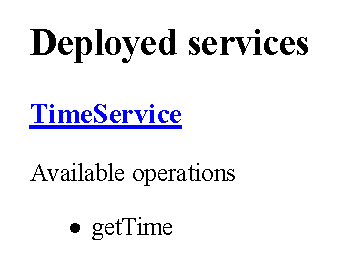
\includegraphics[width=3cm]{figures/axis2-success.pdf}
\end{center}

\subsection{Sample 1: Open Proxy}
\label{sec:sample-1}
We'll start with a very simple configuration that basically does nothing except
logging any incoming messages, then sends the messages to their implicit
destination. Implicit means that Synapse must be able to automatically
determine the final destination of the message based on the message contents,
URL, SOAP header properties, or some other bits of information that are attached to
the message.
\begin{itemize}
  \item Run \texttt{synapse-1.2/bin/synapse -sample 1}
\end{itemize}

\lstset{caption=Open proxy configuration, label=sample-1-xml}
\lstinputlisting{listings/synapse_sample_1.xml}

Now start up SoapUI and create a new project. Enter a project name and use
\url{http://localhost:9000/soap/TimeService?wsdl} as the initial WSDL.
Create a test suite for the imported WSDL. Now go to the preferences and make
SoapUI connect through the Synapse proxy at localhost:8280.

\begin{center}
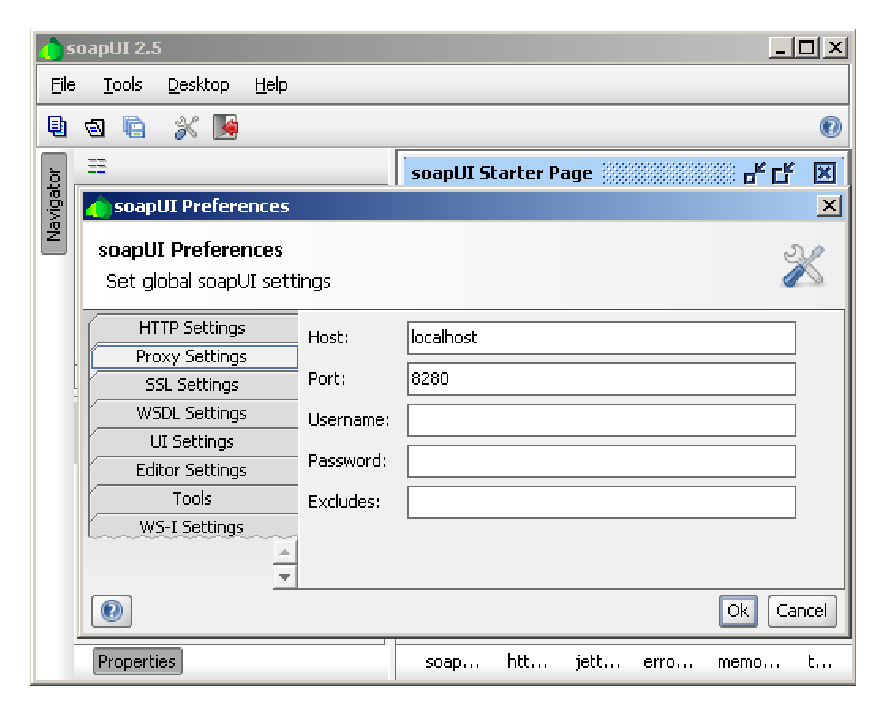
\includegraphics[width=10cm]{figures/soapui-proxy.pdf}
\end{center}

Now you may run the test suite. Your SOAP response should look similar to this: 

\lstset{caption=Open proxy configuration, label=sample-1-xml}
\begin{lstlisting}
<soapenv:Envelope xmlns:soapenv="http://www.w3.org/2003/05/soap-envelope">
   <soapenv:Body>
      <ns:getTimeResponse xmlns:ns="http://esb.seminar.decidr.de">
         <ns:return>2009-01-05T06:42:24.832Z</ns:return>
      </ns:getTimeResponse>
   </soapenv:Body>
</soapenv:Envelope>
\end{lstlisting}

Since the other samples communicate directly with the ESB you should remove the
proxy settings now.

\subsection{Sample 2: Creating a Simple Service Gateway}
\label{sec:sample-2}

\subsection{Sample 3: Service Gateyway with Load Balancing}
\label{sec:sample-3}

\subsection{Sample 4: Service Gateyway with Load Balancing, Reliable Messaging
and Security}
\label{sec:sample-4}

%\newpage
\section{Web Services Security}
\label{chap:web-services-security}
\todo{Explain what WS-Security is. Who developed it? What does it
specify? Explain how it is related to WS-* and web service
technology in general.}

%\newpage
\subsection{Comparison to Transport Layer Security}
\label{sec:comparison-to-transport-layer-securtiy}
\todo{What's the difference between using WS-Security and using HTTPS?}

%\newpage
\subsection{WS-Security Usage in DecidR}
\label{subsec:ws-security-usage-in-decidr}
\todo{Why and where does Decidr require the usage of WSS?}

%\newpage
\subsubsection{Example WS-Security Usage}
\label{subsec:example-ws-security-usage}
\todo{Shows how WS-Security is applied to SOAP messages to provide end-to-end
security, referencing chapter \ref{chap:example-esb-usage}. }
